\documentclass[final,1p,times]{elsarticle}
\usepackage{graphicx}
\usepackage{booktabs}
\usepackage{amsmath}
\usepackage{amssymb}
\usepackage{microtype}
\usepackage[hidelinks]{hyperref}
\usepackage{url}
\usepackage{caption}
\usepackage{subcaption}
\usepackage[section]{placeins}
\usepackage{float}
\biboptions{numbers,sort&compress}
\journal{Signal Processing: Image Communication}
\emergencystretch=2em
\microtypesetup{expansion=false}

% Reduce excessive white space caused by float placement
\setcounter{topnumber}{5}
\setcounter{bottomnumber}{5}
\setcounter{totalnumber}{10}
\renewcommand{\topfraction}{0.95}
\renewcommand{\bottomfraction}{0.95}
\renewcommand{\textfraction}{0.02}
\renewcommand{\floatpagefraction}{0.75}
\setlength{\textfloatsep}{10pt plus 2pt minus 2pt}
\setlength{\floatsep}{8pt plus 2pt minus 2pt}
\setlength{\intextsep}{8pt plus 2pt minus 2pt}
\setlength{\abovecaptionskip}{4pt}
\setlength{\belowcaptionskip}{0pt}
\flushbottom

\begin{document}
\begin{frontmatter}

\title{MP-CycleGAN: Multi-Perceptual Constraints for Unpaired Underwater Image Enhancement}

\author[aff1]{Aoqi Li\fnref{fn1}}
\ead{omglaq@gmail.com}

\author[aff2]{Rongzhi Yang\fnref{fn1}}
\ead{rongzhiy2735@gmail.com}

\author[aff1]{Zixuan Yang\fnref{fn1}}
\ead{18003728268@139.com}

\author[aff1]{Chenfu Yang\corref{cor1}}
\ead{yangchengfu@ynnu.edu.cn}

\cortext[cor1]{Corresponding author}
\fntext[fn1]{These authors contributed equally as co-first authors.}

\affiliation[aff1]{organization={Yunnan Normal University},
            city={Kunming},
            postcode={650500},
            country={China}}
\affiliation[aff2]{organization={Xi'an Precision Machinery Research Institute Kunming Branch},
            city={Kunming},
            postcode={650101},
            country={China}}

\begin{abstract}
Underwater image enhancement (UIE) is an important preprocessing step for visual signal processing pipelines used in marine inspection, robotics, and underwater monitoring. Real underwater images suffer from wavelength-dependent absorption and scattering, which often lead to severe color casts, contrast loss, and haze-like degradation. While supervised UIE models can achieve strong full-reference scores, they rely on paired data that are difficult to collect and may generalize poorly across water conditions. This paper presents MP-CycleGAN, an unpaired UIE framework that regularizes CycleGAN from three complementary perceptual perspectives: a gray-world prior for color balance, gradient consistency for structural stability, and a VGG-based perceptual term for high-level feature preservation. Rather than redesigning the backbone, the proposed method narrows the solution space of unpaired translation through lightweight training-time regularization. We evaluate the method with a unified inference and evaluation pipeline on EUVP (in-domain) and UIEB (cross-domain), and report 95\% bootstrap confidence intervals for PSNR/SSIM together with paired delta analysis. Under a same-budget continuation protocol on the full EUVP matched test subset, MP-CycleGAN shows a stable in-domain PSNR improvement relative to a CycleGAN baseline continued for the same additional training budget, while SSIM changes remain modest and not statistically significant. On cross-domain UIEB testing, MP-CycleGAN also improves full-reference PSNR/SSIM over the same-budget continuation baseline, but the no-reference trends remain mixed, so the domain-shift analysis is still interpreted conservatively rather than as a claim of uniform superiority. These results support MP-CycleGAN as a practical regularization strategy for stabilizing unpaired UIE, while also highlighting the limits of metric agreement and task transfer under domain shift.
\end{abstract}

\begin{keyword}
underwater image enhancement \sep image restoration \sep visual signal processing \sep unpaired learning \sep CycleGAN \sep perceptual regularization
\end{keyword}

\end{frontmatter}

\section{Introduction}
Underwater imagery is widely used in marine exploration, infrastructure inspection, ecological monitoring, and robot navigation. In such systems, UIE is not only a visual enhancement problem but also a pre-processing stage for downstream visual signal processing tasks such as detection, recognition, and communication-oriented image analysis. Because light is selectively absorbed and scattered in water, underwater images often exhibit severe color casts, low contrast, veiling light, and detail attenuation, all of which degrade both human interpretability and machine perception.

Supervised deep UIE models can perform well when trained on aligned underwater/clean pairs, but collecting such pairs in real marine environments is difficult and expensive. Synthetic pairs partially alleviate this issue, yet domain gaps across water types, illumination, and camera settings often limit generalization. Unpaired translation methods such as CycleGAN~\cite{zhu2017cyclegan} are therefore attractive in practice because they reduce the dependence on aligned supervision. However, the mapping learned in unpaired settings is ill-posed and can easily drift toward visually plausible but structurally unstable or color-biased solutions. In underwater scenes, this instability typically appears as residual blue/green casts, distorted edges, or hallucinated textures.

From this perspective, the central question of this paper is not whether a standard unpaired backbone can be replaced by a larger architecture, but whether it can be regularized more effectively during training. We therefore study a lightweight refinement strategy for CycleGAN in which three failure modes of unpaired UIE are addressed jointly: color instability, structural drift, and feature inconsistency. The proposed MP-CycleGAN introduces a gray-world prior, a gradient-consistency term, and a VGG-based perceptual constraint during training only. The intended effect is to narrow the feasible solution space of unpaired translation and move the model toward a more stable operating point, while leaving the inference-time backbone unchanged.

\noindent\textbf{Contributions.} The main contributions of this work are as follows. First, we formulate a training-time regularization strategy for unpaired UIE that combines complementary color, structural, and feature-space perceptual constraints without changing the inference-time architecture. Second, we establish a unified evaluation protocol on EUVP and UIEB, report 95\% bootstrap confidence intervals for PSNR/SSIM, and organize per-image metrics so that paired delta analysis can be reproduced directly under the same-budget continuation setting used for the final unpaired comparison. Third, we position the empirical findings conservatively through matched-set, cross-domain, and downstream detection analyses, showing a modest in-domain PSNR-oriented refinement signal together with cross-domain metric trade-offs and task-level domain-shift effects.

\section{Related Work}
UIE methods can be broadly categorized into prior-based restoration, supervised deep learning, and unpaired or weakly supervised translation. Classical prior-based methods typically exploit hand-crafted assumptions about underwater image formation or visual statistics. Representative examples include wavelength-compensation and dehazing strategies~\cite{chiang2012wavelength}, fusion-based enhancement~\cite{ancuti2012fusion}, blur-and-absorption modeling~\cite{peng2017blurriness}, and water-removal methods that explicitly estimate scene-dependent attenuation~\cite{akkaynak2019seathru}. These approaches are often interpretable and physically motivated, but their assumptions may not hold uniformly across different water bodies and imaging conditions.

Supervised deep models learn a direct mapping from degraded inputs to reference images or synthetic targets. Benchmark-driven works such as UIEB~\cite{li2020uieb}, FUnIE-GAN~\cite{islam2020funiegan}, and UColor~\cite{li2021ucolor} demonstrate that learned models can achieve strong quantitative performance when paired supervision or synthetic references are available. More recent UIE studies have also explored stronger backbones and alternative learning paradigms, including adaptive normalization and cascaded attention CNNs~\cite{park2024asnet,zhang2024cnms}, transformer- and diffusion-based designs~\cite{tang2023diffusion,ding2025aldiff}, and lightweight zero-reference enhancement~\cite{liu2024zerouae}. Nevertheless, collecting strictly aligned underwater/clean pairs remains difficult, and the resulting models may be sensitive to domain gaps between training and deployment. In addition, the objectives used in many of these methods are optimized with access to paired references, synthetic surrogates, or image-specific adjustment targets, which is a weaker assumption than the fully unpaired setting considered here.

Unpaired and adversarial methods are attractive when paired supervision is unavailable. UGAN~\cite{fabbri2018ugan} and CycleGAN-style translation~\cite{zhu2017cyclegan} reduce the dependence on aligned pairs by combining adversarial learning with reconstruction constraints. Their main limitation is that the learned mapping can still be under-constrained: adversarial realism alone does not guarantee stable color correction, structural fidelity, or feature-space consistency. Recent unsupervised or weakly supervised UIE variants have therefore introduced additional priors and adversarial constraints such as edge extraction, self-adversarial quality transfer, and enhanced generator modules~\cite{jia2024unsupervised,wang2024sagan}. More generally, perceptual and feature-space objectives have long been used to stabilize image transformation problems~\cite{johnson2016perceptual}, while gray-world assumptions remain a classic cue for color correction in degraded visual environments~\cite{buchsbaum1980grayworld}. Our work follows this regularization-oriented line rather than proposing a new backbone. The key difference is that we integrate color, structure, and feature-space perceptual constraints into a unified training-time design for unpaired UIE, and we evaluate the resulting trade-offs under matched-set, cross-domain, and task-driven protocols. This positioning is important: the contribution of MP-CycleGAN is not a new generator architecture, but a practical way to make unpaired enhancement more stable and more interpretable.

This distinction also aligns with recent reviews of the field. Recent surveys and benchmarking studies note that UIE research is moving toward larger backbones, broader learning paradigms, and more diverse evaluation protocols, while still facing unresolved issues in generalization, metric mismatch, and deployment-oriented assessment~\cite{cong2024survey,lai2025review,shen2025uiqe,liu2024uiqa}. In this context, our goal is deliberately narrower: instead of competing with every new architecture family, we study whether a lightweight regularization strategy can make a standard unpaired framework behave more stably across matched-set, cross-domain, and downstream settings.

\section{Method}
\subsection{CycleGAN Base}
We consider two domains: underwater images $A$ and enhanced (clear) images $B$. CycleGAN learns two generators $G: A\rightarrow B$ and $F: B\rightarrow A$ with two discriminators $D_B$ and $D_A$. For visual clarity, Fig.~\ref{fig:method_overview} highlights the $A\rightarrow B\rightarrow A$ branch and the discriminator $D_B$; the reverse branch and $D_A$ are symmetric and omitted from the drawing. The objective includes adversarial losses and cycle-consistency:
\begin{equation}
\mathcal{L}_{total}=\mathcal{L}_{GAN}+\lambda_{cyc}\mathcal{L}_{cyc}+\lambda_{idt}\mathcal{L}_{idt}+\mathcal{L}_{MP}.
\end{equation}

\begin{figure}[!t]
\centering
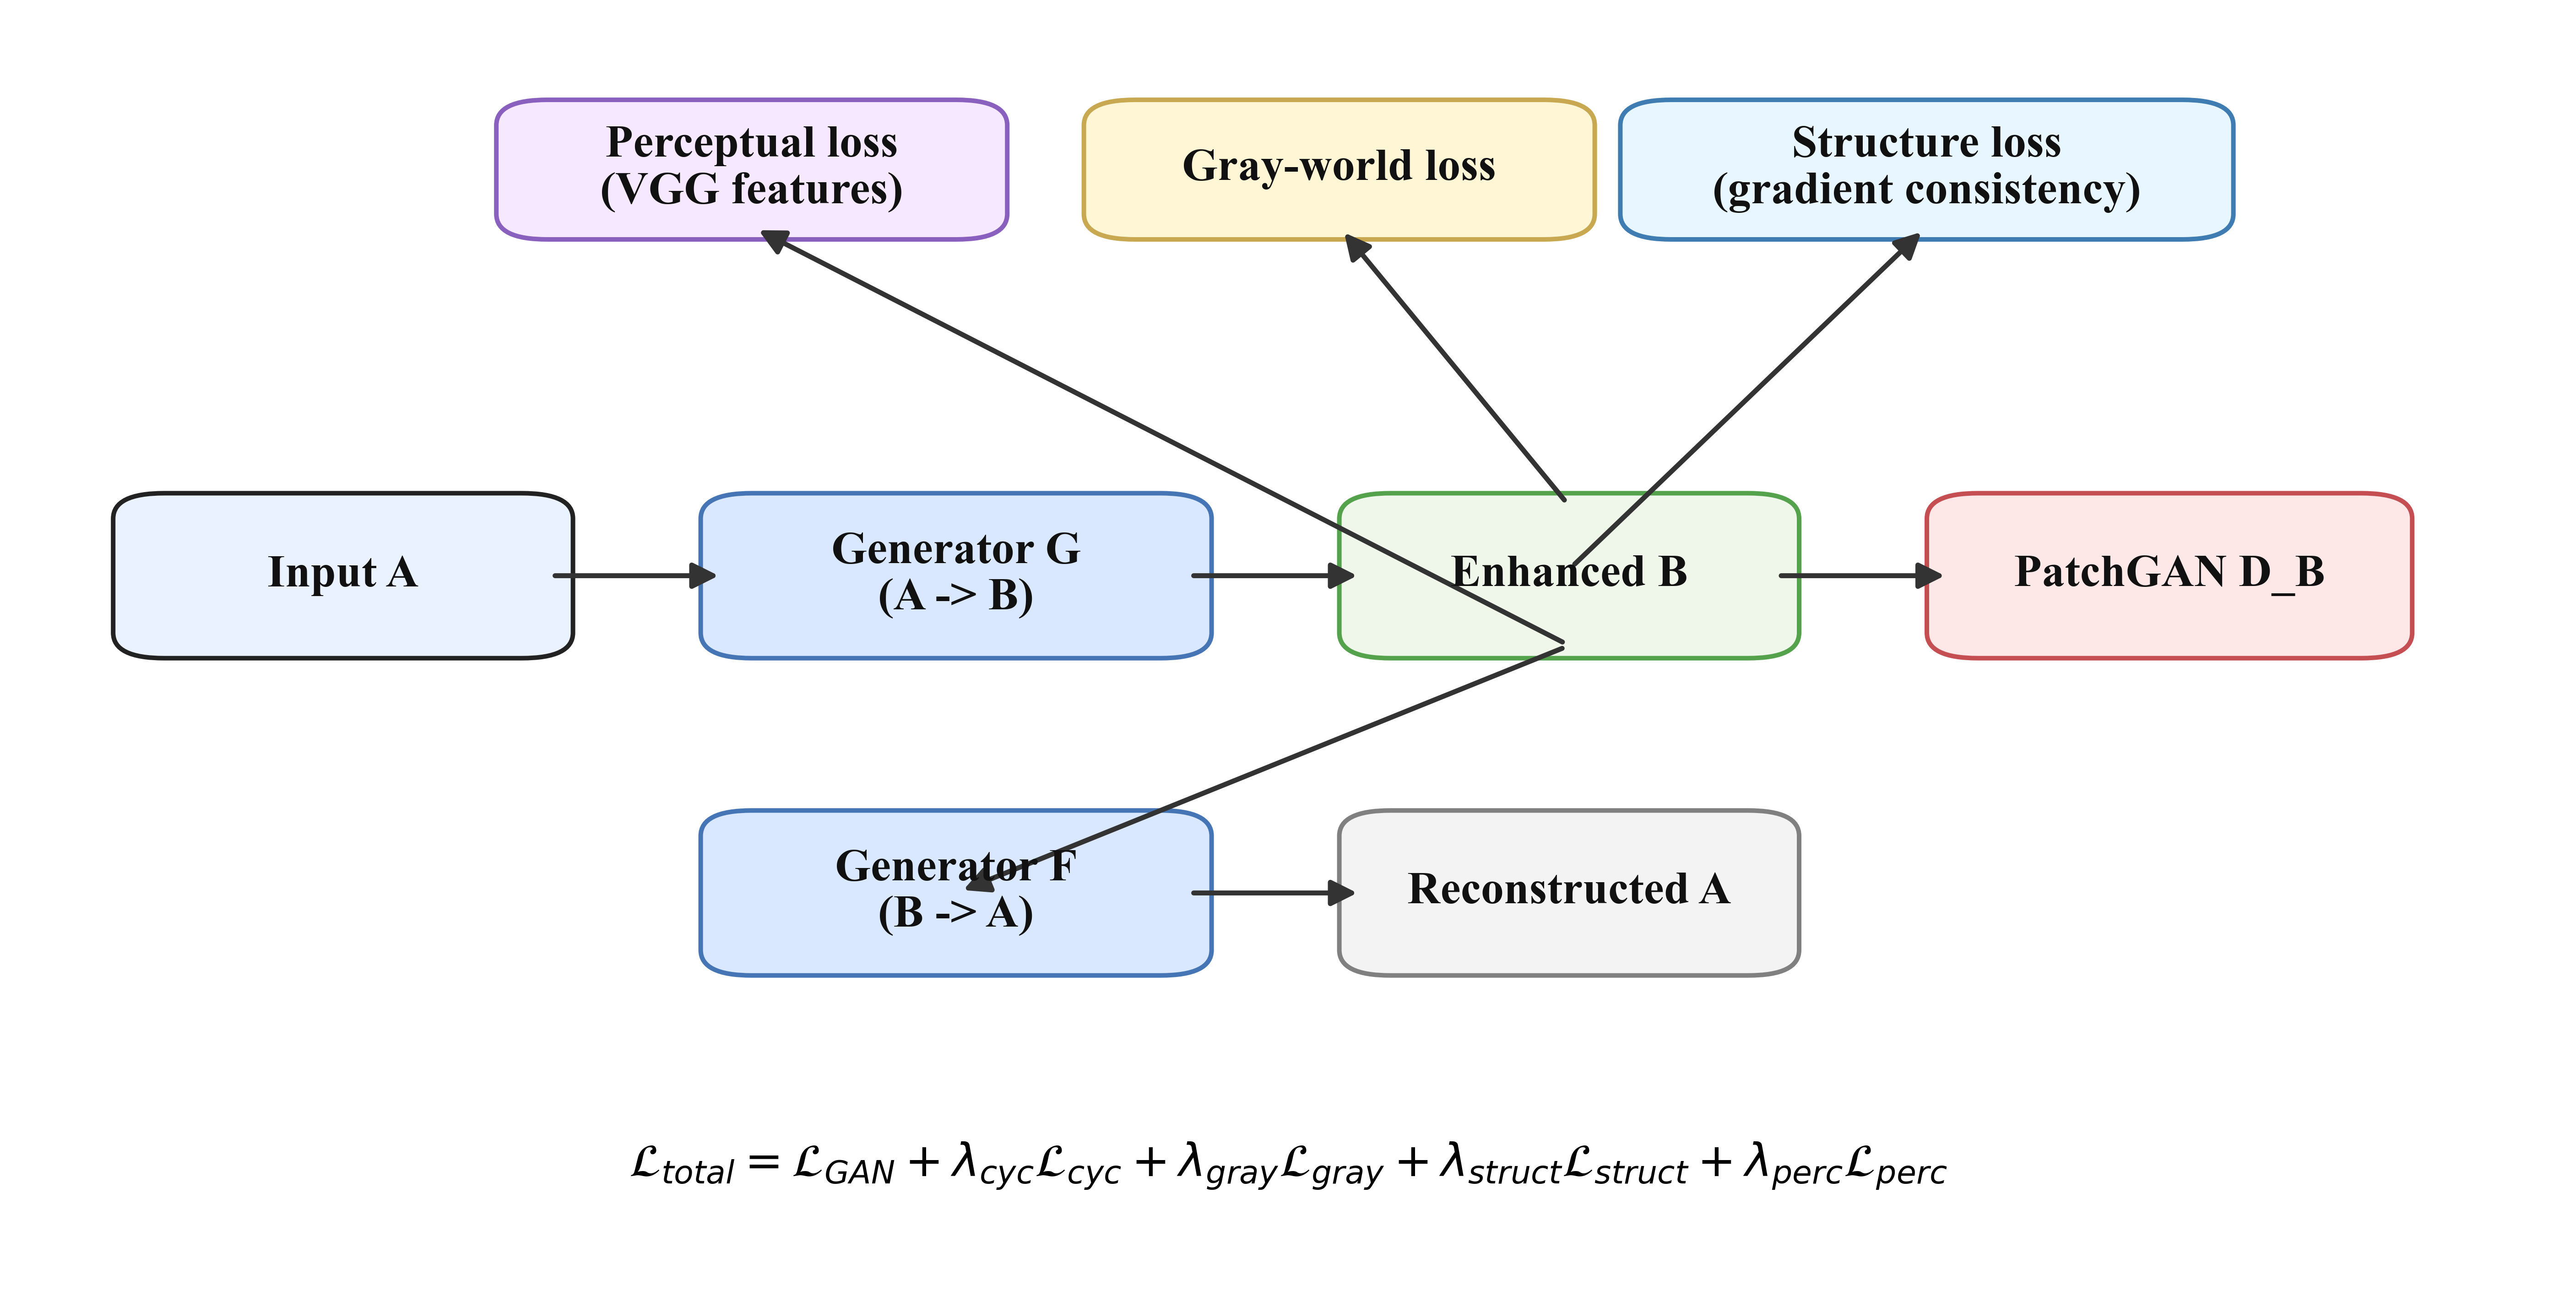
\includegraphics[width=0.95\linewidth]{figures_used/Fig1_method_overview_spic.png}
\caption{Overview of the proposed MP-CycleGAN framework. The figure highlights the $A\rightarrow B\rightarrow A$ branch, where the generated enhanced image is regularized by the gray-world prior, gradient-based structure consistency, and VGG-based perceptual consistency. These MP constraints are applied only during training and do not change inference-time complexity.}
\label{fig:method_overview}
\end{figure}

\subsection{Multi-Perceptual Constraints (MP)}
In this paper, MP denotes three complementary perceptual perspectives used to regularize unpaired UIE. As illustrated in Fig.~\ref{fig:method_overview}, all three terms are attached to the generated enhanced output and act as training-time regularizers rather than inference-time modules:
\begin{equation}
\mathcal{L}_{MP}=\lambda_{gray}\mathcal{L}_{gray}+\lambda_{struct}\mathcal{L}_{struct}+\lambda_{perc}\mathcal{L}_{perc}.
\end{equation}
\paragraph{Color perception: gray-world prior.}
We use a differentiable gray-world loss to encourage balanced RGB channel means in the enhanced output $\hat{I}$:
\begin{equation}
\mathcal{L}_{gray}(\hat{I})=\frac{1}{3}\sum_{c\in\{r,g,b\}}\left|\mu_c(\hat{I})-\mu_{gray}(\hat{I})\right|,\quad
\mu_{gray}(\hat{I})=\frac{\mu_r(\hat{I})+\mu_g(\hat{I})+\mu_b(\hat{I})}{3}.
\end{equation}
\paragraph{Structure perception: gradient consistency.}
To reduce structural drift during translation, we constrain first-order gradients between the input $I$ and output $\hat{I}$:
\begin{equation}
\mathcal{L}_{struct}(I,\hat{I})=\left\|\nabla_x \hat{I}-\nabla_x I\right\|_1+\left\|\nabla_y \hat{I}-\nabla_y I\right\|_1.
\end{equation}
\paragraph{Feature-space perception: VGG perceptual loss.}
We use a VGG-16 feature extractor $\phi$ to align input and output in feature space:
\begin{equation}
\mathcal{L}_{perc}(I,\hat{I})=\left\|\phi(I)-\phi(\hat{I})\right\|_1.
\end{equation}

\paragraph{Auxiliary color-statistics regularizer.}
In a separate exploratory ablation, we additionally test a global color-statistics term that matches the mean and standard deviation of the generated output to those of the input:
\begin{equation}
\mathcal{L}_{color}(I,\hat{I})=\left\|\mu(\hat{I})-\mu(I)\right\|_1+\left\|\sigma(\hat{I})-\sigma(I)\right\|_1.
\end{equation}
This auxiliary term is not part of the default MP-CycleGAN definition reported in the main comparisons; it is only used to examine whether an extra global color constraint changes the metric trade-off in the ablation study.

\section{Experiments}
\subsection{Datasets and Protocol}
\textbf{EUVP (in-domain).} The main models are trained on the unpaired branch of EUVP and evaluated on the matched subset \texttt{test\_samples} (matched=515). During evaluation, each input image is translated only once through $G: A\rightarrow B$, and the enhanced result is compared against the aligned reference for PSNR/SSIM. UCIQE and UIQM are computed on the predicted images to reflect no-reference quality tendencies.

For the final fairness control, we use a same-budget continuation protocol on the full matched test subset. Specifically, the selected CycleGAN epoch200 checkpoint is further continued to epoch250, and MP-CycleGAN is refined from the same epoch200 initialization to epoch250 under the same additional training budget. The in-domain paired delta analysis is therefore reported on the full 515-image matched subset rather than on the earlier archived 200-image export.

\textbf{UIEB (cross-domain).} To test cross-domain generalization, the EUVP-trained models are directly applied to UIEB without any UIEB fine-tuning. Full-reference and no-reference metrics are computed on the 841-image matched subset retained after filename intersection between the available UIEB inputs and reference files in the current benchmark export. For paired PSNR/SSIM delta analysis, 23 rows with missing full-reference values in both benchmark CSV files are excluded, leaving 818 valid pairs. Because UIEB references are collected under a different acquisition protocol, cross-domain PSNR/SSIM and no-reference metrics are expected to reflect partially different preferences rather than identical rankings.

\subsection{Metrics and Reproducibility}
We report PSNR/SSIM as full-reference metrics and UCIQE/UIQM as no-reference metrics. For PSNR/SSIM, we report 95\% bootstrap confidence intervals computed by repeated resampling (\texttt{bootstrap\_iters=2000}, \texttt{seed=123}). The confidence intervals are used to describe the stability of the mean estimates on matched subsets; they should therefore be interpreted as uncertainty ranges for the reported averages, not as proof that every small numerical difference is practically significant. The evaluation pipeline also exports per-image metrics, which makes paired delta analysis such as median improvement, win rate, and Wilcoxon signed-rank testing directly reproducible from the released CSV files.

\subsection{Implementation Notes}
At inference time, only $G: A\rightarrow B$ is used. MP constraints are applied only during training and do not add runtime modules at inference. The baseline CycleGAN model follows the standard configuration of the official implementation: ResNet-9 generator, basic PatchGAN discriminator, Adam optimizer with $\beta_1=0.5$, learning rate $2\times10^{-4}$, \texttt{n\_epochs}=100, \texttt{n\_epochs\_decay}=100, \texttt{batch\_size}=1, and \texttt{resize\_and\_crop} preprocessing with \texttt{load\_size}=286 and \texttt{crop\_size}=256. For the final fairness control, the selected CycleGAN epoch200 checkpoint is continued to epoch250 with learning rate $1\times10^{-4}$ and \texttt{max\_dataset\_size}=500. MP-CycleGAN is initialized from the same epoch200 checkpoint and refined to epoch250 under the same continuation budget with $\lambda_{gray}=0.1$, $\lambda_{struct}=2.0$, $\lambda_{perc}=0.05$, \texttt{perceptual\_layer}=16, and $\lambda_{color}=0.0$ in the default model. The main paired analyses are therefore based on a same-budget epoch250 continuation setting.

\textbf{Baseline fairness.} The main claim is intentionally narrow. CycleGAN and MP-CycleGAN share the same backbone family, image resolution, and metric scripts, and the cross-domain UIEB evaluation uses no UIEB fine-tuning for either model. In the final unpaired comparison, both models are evaluated after the same additional continuation budget from the same epoch200 initialization, so MP-CycleGAN should be read as a lightweight stage-two regularization derived from a controlled same-budget baseline rather than as a claim that a new generator architecture replaces all existing UIE families. CUT and FastCUT are treated as external unpaired baselines trained on the same EUVP unpaired split and re-evaluated using the same post-processing and metric scripts. We additionally report UGAN-P and FUnIE-GAN as contextual paired baselines trained on the EUVP paired split. Because they use paired supervision, they are not used to support strict same-supervision fairness claims against the unpaired main methods.

\subsection{Model Complexity and Runtime}
\begin{table}[!t]
\centering
\caption{Inference-time complexity of the main unpaired models. Because the MP constraints are used only during training, MP-CycleGAN keeps the same inference-time backbone as CycleGAN.}
\label{tab:complexity}
\begin{tabular}{lccc}
\toprule
Method & Generator Params (M) & Runtime (ms/img) & Extra inference cost \\
\midrule
CycleGAN & 11.38 & 17 & No \\
MP-CycleGAN & 11.38 & 17 & No \\
\bottomrule
\end{tabular}
\end{table}
We use the standard CycleGAN backbone (ResNet-9 generator and PatchGAN discriminator). The ResNet-9 generator has approximately 11.38M parameters. For a $256\times256$ input with batch size 1, the average inference time of the generator is about 17 ms per image on an NVIDIA RTX 3060 Laptop GPU (PyTorch 2.5.1, CUDA 12.1). Because the added MP terms appear only in the training objective, the proposed method does not introduce extra inference-time modules, parameters, or post-processing steps. We report these numbers for reference and note that runtime can vary across hardware and software environments.

\section{Results}
\subsection{In-domain Quantitative Results (EUVP)}
\begin{table}[!t]
\centering
\caption{In-domain results on the EUVP matched test subset (matched=515). PSNR/SSIM are reported as mean $\pm$ half-width of the 95\% bootstrap CI (computed on matched pairs). The main claim is based on same-budget unpaired baselines evaluated under the same post-processing and metric scripts.}
\begin{tabular}{lcccc}
\toprule
Method & PSNR (dB) & SSIM & UCIQE & UIQM \\
\midrule
Identity & 20.33$\pm$0.39 & 0.794$\pm$0.008 & 24.88 & 5.77 \\
Gray-World & 19.42$\pm$0.43 & 0.784$\pm$0.009 & 24.27 & 6.72 \\
CycleGAN (+50-epoch continuation) & 22.64$\pm$0.27 & 0.789$\pm$0.006 & 26.78 & 5.39 \\
CUT (external, epoch200) & 21.73$\pm$0.36 & 0.748$\pm$0.010 & 27.56 & 5.17 \\
FastCUT (external, epoch200) & 22.29$\pm$0.41 & 0.764$\pm$0.010 & 26.83 & 5.59 \\
MP-CycleGAN (+50-epoch refinement) & \textbf{22.76$\pm$0.27} & \textbf{0.790$\pm$0.006} & 25.64 & 5.39 \\
\midrule
UGAN-P (paired, epoch200) & \textbf{24.27$\pm$0.26} & \textbf{0.827$\pm$0.005} & 27.44 & 5.29 \\
FUnIE-GAN (paired, epoch200) & 23.19$\pm$0.24 & 0.782$\pm$0.006 & 27.08 & \textbf{5.10} \\
\bottomrule
\end{tabular}
\vspace{2pt}

\footnotesize
$\dagger$ External baselines evaluated using the same post-processing and metric scripts on the final benchmark export.\\
$\ddagger$ Paired supervised models included strictly for contextual reference.
\end{table}

\begin{table}[!t]
\centering
\caption{Paired delta analysis of MP-CycleGAN relative to the same-budget CycleGAN continuation baseline. Positive deltas indicate improvement of MP-CycleGAN over the baseline. For UIEB, 23 rows with missing full-reference values in both benchmark CSV files are excluded, leaving 818 valid paired samples for the paired test.}
\label{tab:paired_delta}
\begin{tabular}{llcccc}
\toprule
Dataset & Metric & Mean $\Delta$ & Median $\Delta$ & Win rate & Wilcoxon $p$ \\
\midrule
EUVP & PSNR & $+0.12$ & $+0.14$ & 57.1\% & 0.0015 \\
EUVP & SSIM & $+0.0016$ & $+0.0012$ & 53.0\% & 0.211 \\
UIEB & PSNR & $+0.08$ & $+0.04$ & 54.9\% & 0.00049 \\
UIEB & SSIM & $+0.0042$ & $+0.0025$ & 58.2\% & $<0.0001$ \\
\bottomrule
\end{tabular}
\end{table}

Within the same-budget unpaired comparison set, MP-CycleGAN improves the mean PSNR from 22.64 dB to 22.76 dB and the mean SSIM from 0.789 to 0.790 relative to the CycleGAN continuation baseline on the full EUVP matched subset. The gain remains numerically modest, and the confidence intervals show that the two unpaired models remain close. The paired statistics in Table~\ref{tab:paired_delta} nevertheless sharpen the interpretation of this small difference. For PSNR, the average delta is $+0.12$ dB, the median delta is $+0.14$ dB, the win rate is $57.1\%$, and the Wilcoxon signed-rank test supports a stable positive shift ($p=0.0015$). For SSIM, by contrast, the average delta is only $+0.0016$, the median delta is $+0.0012$, the win rate is $53.0\%$, and the Wilcoxon test does not support a clear shift ($p=0.211$). We therefore interpret the final fairness-controlled result conservatively: under a matched additional training budget, the proposed constraints provide a small but statistically supported PSNR-oriented refinement, while SSIM gains are weak and should not be overstated.

For contextual reference, the paired UGAN-P baseline reaches 24.27 dB PSNR and 0.827 SSIM on the same matched subset, while paired FUnIE-GAN reaches 23.19 dB PSNR and 0.782 SSIM with a mean UCIQE of 27.08. Both paired baselines benefit from stronger supervision than the unpaired methods in the main comparison, but only UGAN-P clearly exceeds the unpaired models in full-reference fidelity. We therefore treat both rows as contextual references rather than as evidence against the main unpaired claim.

The no-reference metrics also reveal that not every prior is beneficial in the same way. For example, Gray-World increases UIQM but performs worse in PSNR/SSIM, suggesting that a simple color-balancing heuristic can improve perceptual contrast while still deviating from the matched references. This contrast helps motivate the proposed combination of priors and learned translation: the objective is to improve stability without sacrificing the reconstruction behavior learned by CycleGAN.

\begin{figure}[!t]
\centering
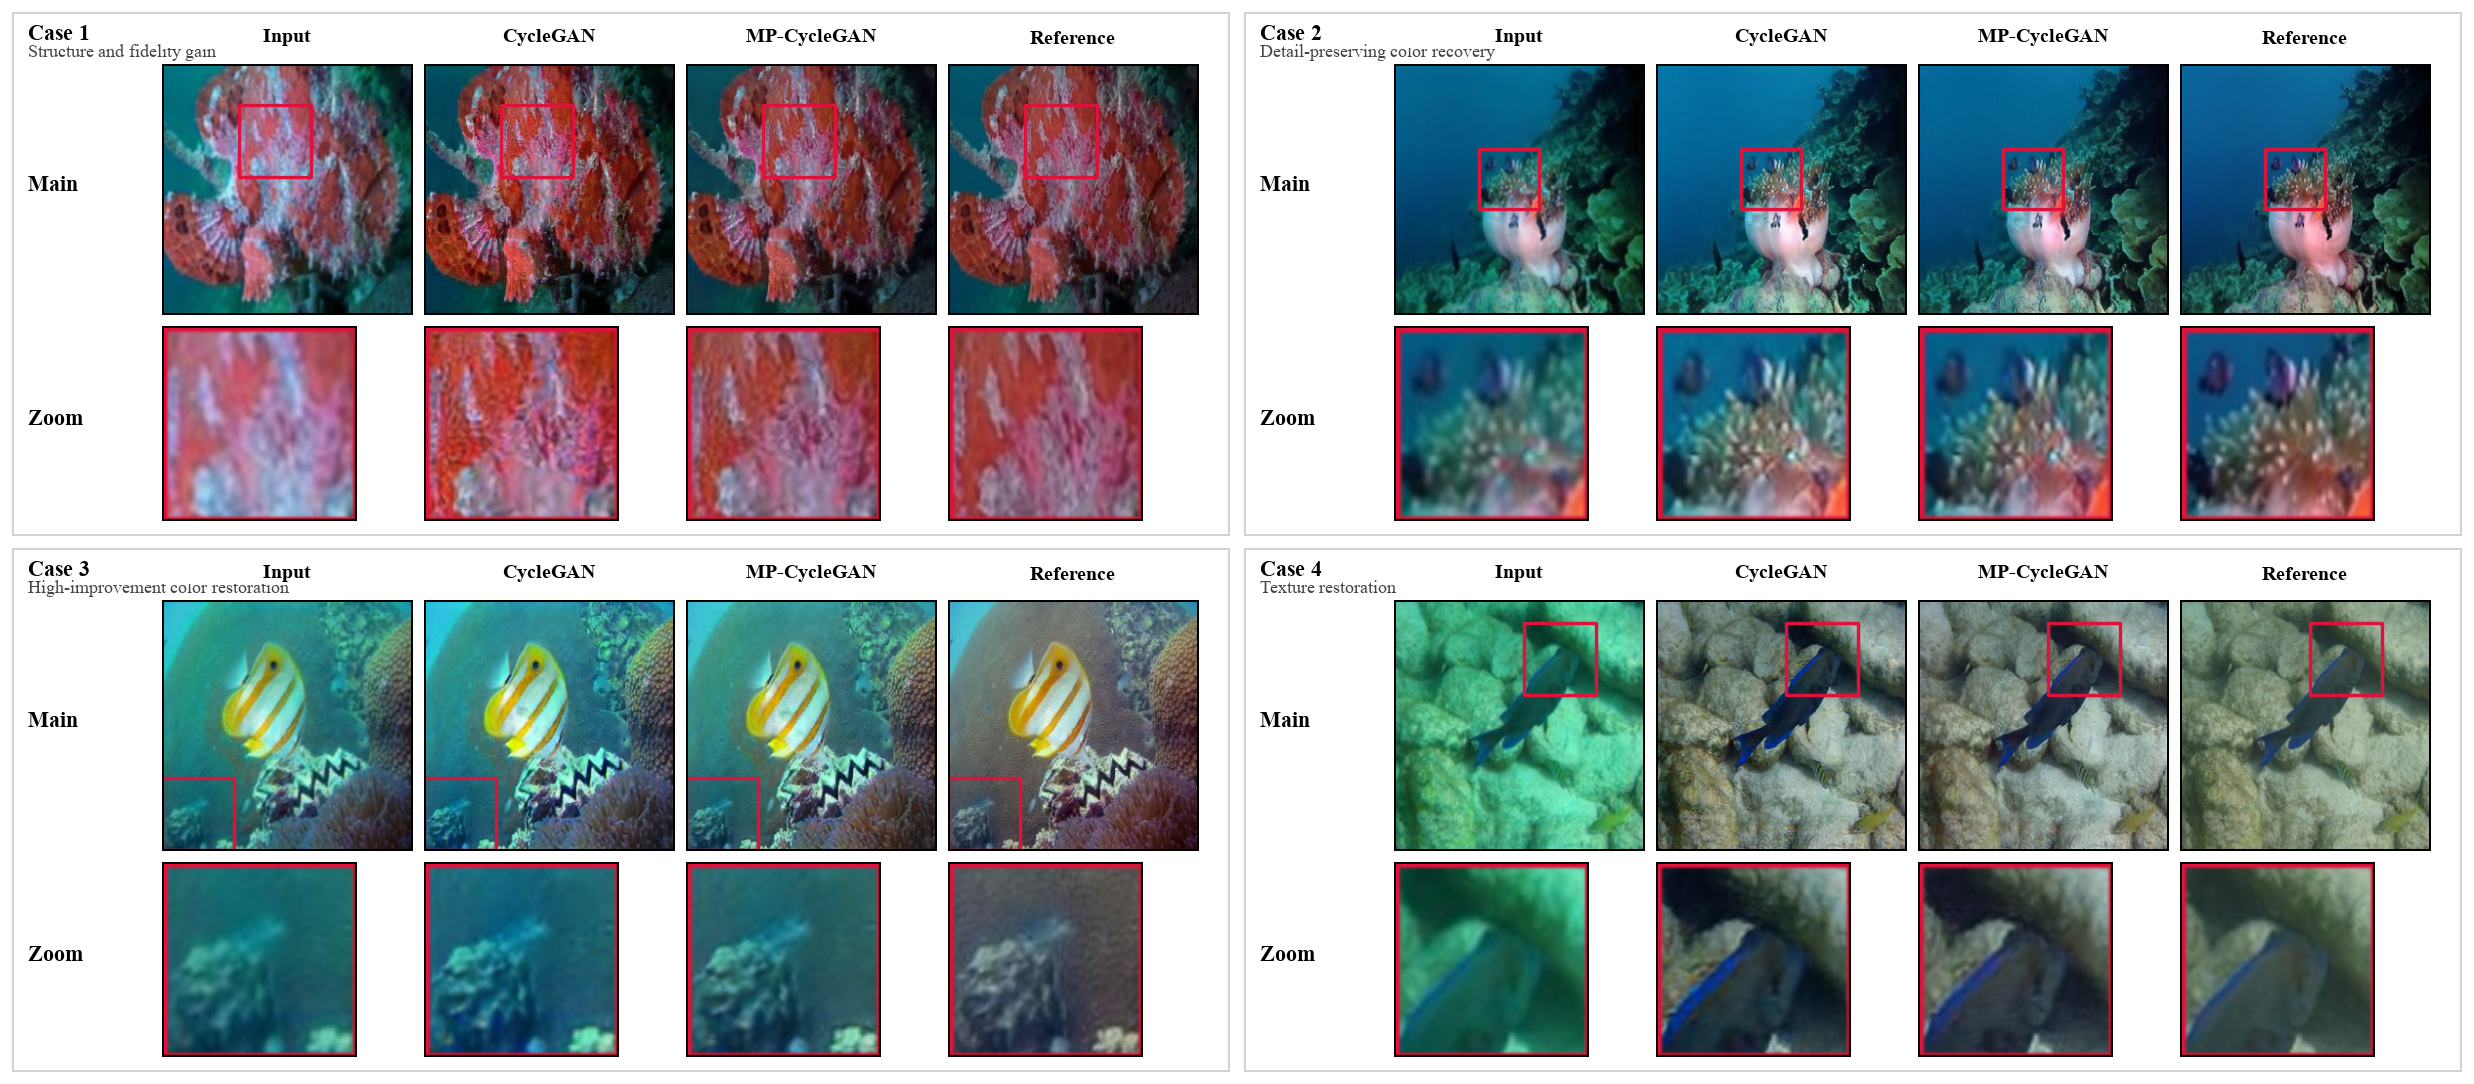
\includegraphics[width=0.98\linewidth]{figures_used/Fig2_euvp_in_domain_qualitative_spic.png}
\caption{In-domain qualitative comparison on EUVP under the final same-budget 250 vs 250 setting (input, CycleGAN continuation, MP-CycleGAN refinement, reference). The displayed cases are representative examples identified from paired per-image analysis while maintaining visible differences in structure, color, and texture recovery.}
\end{figure}

Competitive scalar scores do not always imply locally faithful enhancement. To probe this point more directly, Fig.~\ref{fig:cut_counterexample} presents two hard EUVP cases selected from the paired per-image export where CUT and FastCUT show clear local failure modes while MP-CycleGAN remains more stable. In Case 1, which contains elongated rigid edges and junction topology, both CUT variants introduce halo-like dark bands and local edge warping around the diver-equipment boundary. In Case 2, which contains dense coral texture, CUT and FastCUT amplify blotchy texture and false speckle patterns that are less consistent with the reference appearance. By contrast, MP-CycleGAN preserves cleaner contours and smoother local shading in both cases without changing the inference-time backbone. This comparison is not meant to override the quantitative tables; rather, it explains why competitive global metrics from contrast-oriented unpaired baselines should still be interpreted together with localized structural fidelity.

\begin{figure}[!t]
\centering
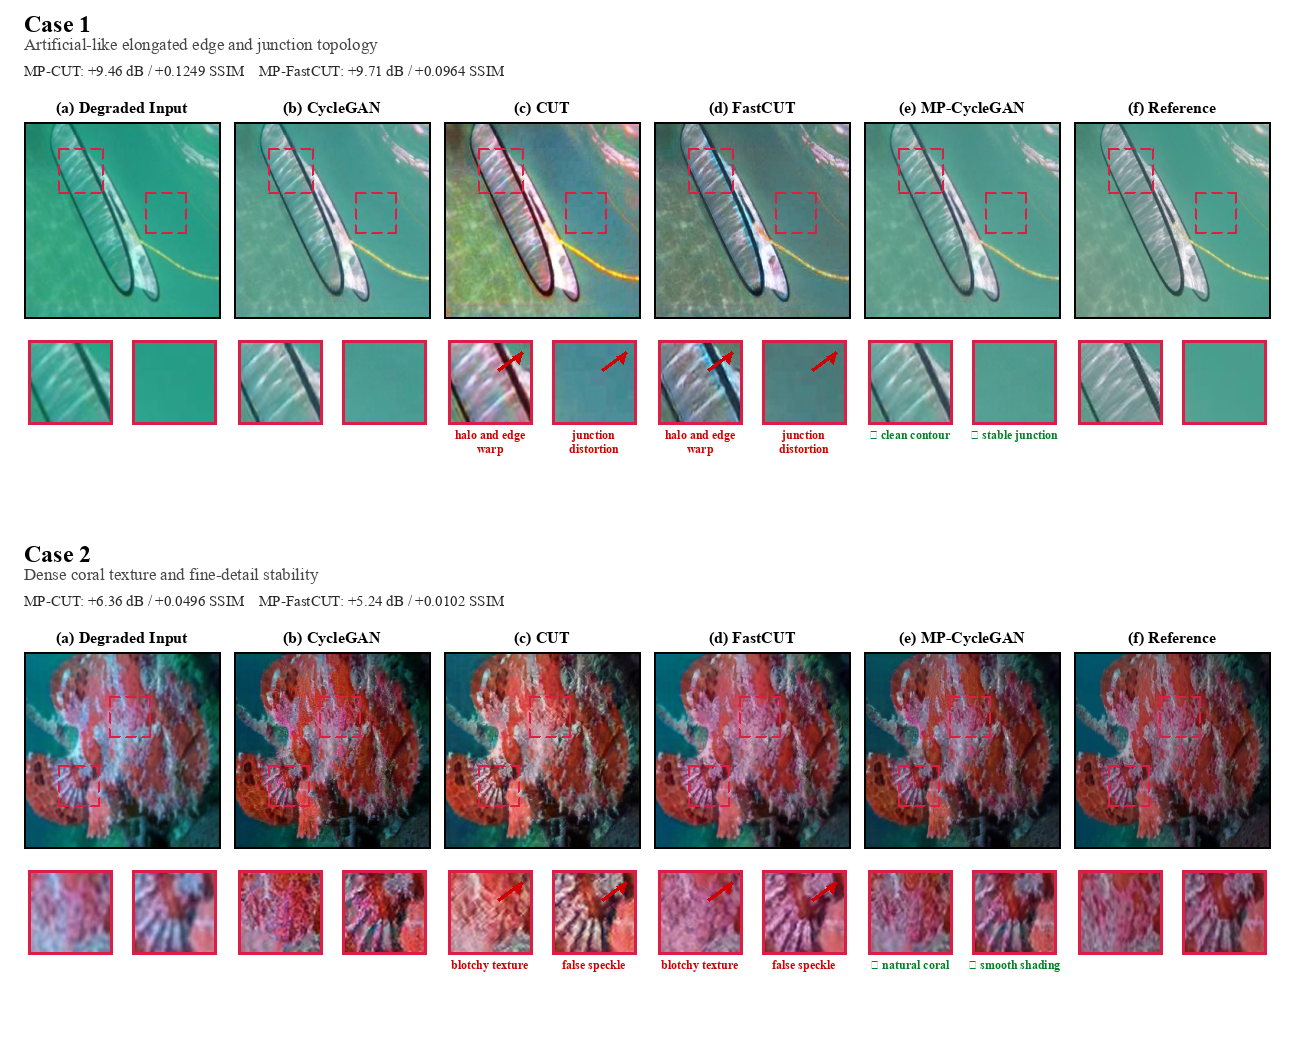
\includegraphics[width=0.99\linewidth]{figures_used/Fig_cut_fastcut_counterexample_spic.png}
\caption{Reviewer-oriented qualitative counterexamples against CUT and FastCUT on EUVP. The two cases are selected from the paired per-image export to stress scenarios where local fidelity matters: Case 1 focuses on rigid elongated edges and junction topology, and Case 2 focuses on dense coral texture and fine-detail stability. Red boxes indicate the shared zoom regions across all methods; red arrows mark local artifacts in CUT/FastCUT such as halo-like edge warping, junction distortion, blotchy texture, and false speckle; green labels indicate the corresponding contour and texture preservation of MP-CycleGAN.}
\label{fig:cut_counterexample}
\end{figure}

\subsection[Cross-domain Results (EUVP to UIEB)]{Cross-domain Results (EUVP $\rightarrow$ UIEB)}
\begin{table}[!t]
\centering
\caption{Cross-domain testing on the UIEB matched subset used in the final benchmark export (matched=841). PSNR/SSIM are reported as mean $\pm$ half-width of the 95\% bootstrap CI when available. All methods are evaluated without UIEB fine-tuning; the cross-domain comparison is interpreted as a trade-off analysis rather than a claim of universal superiority.}
\label{tab:uieb_quant}
\begin{tabular}{lcccc}
\toprule
Method & PSNR (dB) & SSIM & UCIQE & UIQM \\
\midrule
Input & - & - & 21.38 & 6.89 \\
\midrule
CycleGAN (+50-epoch continuation)$^\dagger$ & 17.74$\pm$0.20 & 0.637$\pm$0.009 & 23.22 & 10.05 \\
CUT (external)$^\dagger$ & \textbf{18.31$\pm$0.16} & 0.624$\pm$0.009 & \textbf{28.48} & 9.62 \\
FastCUT (external)$^\dagger$ & 17.63$\pm$0.18 & 0.588$\pm$0.009 & 25.37 & 10.06 \\
MP-CycleGAN (+50-epoch refinement)$^\dagger$ & 17.83$\pm$0.20 & 0.641$\pm$0.009 & 22.74 & \textbf{10.10} \\
\midrule
UGAN-P (paired)$^\ddagger$ & 17.96$\pm$0.20 & \textbf{0.674$\pm$0.009} & 25.39 & 9.96 \\
FUnIE-GAN (paired)$^\ddagger$ & 17.25$\pm$0.22 & 0.637$\pm$0.009 & 23.92 & 9.66 \\
\bottomrule
\end{tabular}
\vspace{2pt}

\footnotesize
$\dagger$ Unpaired methods trained on EUVP and evaluated on UIEB without UIEB fine-tuning.\\
$\ddagger$ Paired supervised models trained on EUVP, included strictly for cross-domain contextual reference.
\end{table}

The cross-domain results should be read as a robustness trade-off rather than a uniform win for any single method. On the 841-image UIEB matched subset used in the final benchmark export, the same-budget CycleGAN continuation baseline reaches 17.74 dB PSNR, 0.637 SSIM, UCIQE 23.22, and UIQM 10.05, whereas MP-CycleGAN reaches 17.83 dB PSNR, 0.641 SSIM, UCIQE 22.74, and UIQM 10.10. Thus, under domain shift, the proposed constraints produce modest full-reference gains and a slight UIQM increase, but do not improve UCIQE. For paired delta analysis on UIEB, 23 rows with missing full-reference values in both benchmark CSV files are excluded, leaving 818 valid pairs. On these valid pairs, MP-CycleGAN yields a mean PSNR delta of $+0.08$ dB (median $+0.04$, win rate 54.9\%, Wilcoxon $p=0.00049$) and a mean SSIM delta of $+0.0042$ (median $+0.0025$, win rate 58.2\%, Wilcoxon $p<0.0001$). We therefore keep the cross-domain claim conservative: the UIEB result indicates a modest positive shift in full-reference fidelity under the current domain mismatch, although the effect size remains small in magnitude, and the mixed no-reference behavior shows that this should still be interpreted as a trade-off analysis rather than as evidence of broad superiority across all criteria. For contextual reference, the paired UGAN-P baseline reaches 17.96 dB PSNR and 0.674 SSIM on UIEB, whereas paired FUnIE-GAN reaches 17.25 dB PSNR and 0.637 SSIM with a mean UCIQE of 23.92 and UIQM of 9.66. These paired results again show that stronger supervision can improve some full-reference scores under domain shift, but does not guarantee dominance on all perceptual metrics.

\begin{figure}[!t]
\centering
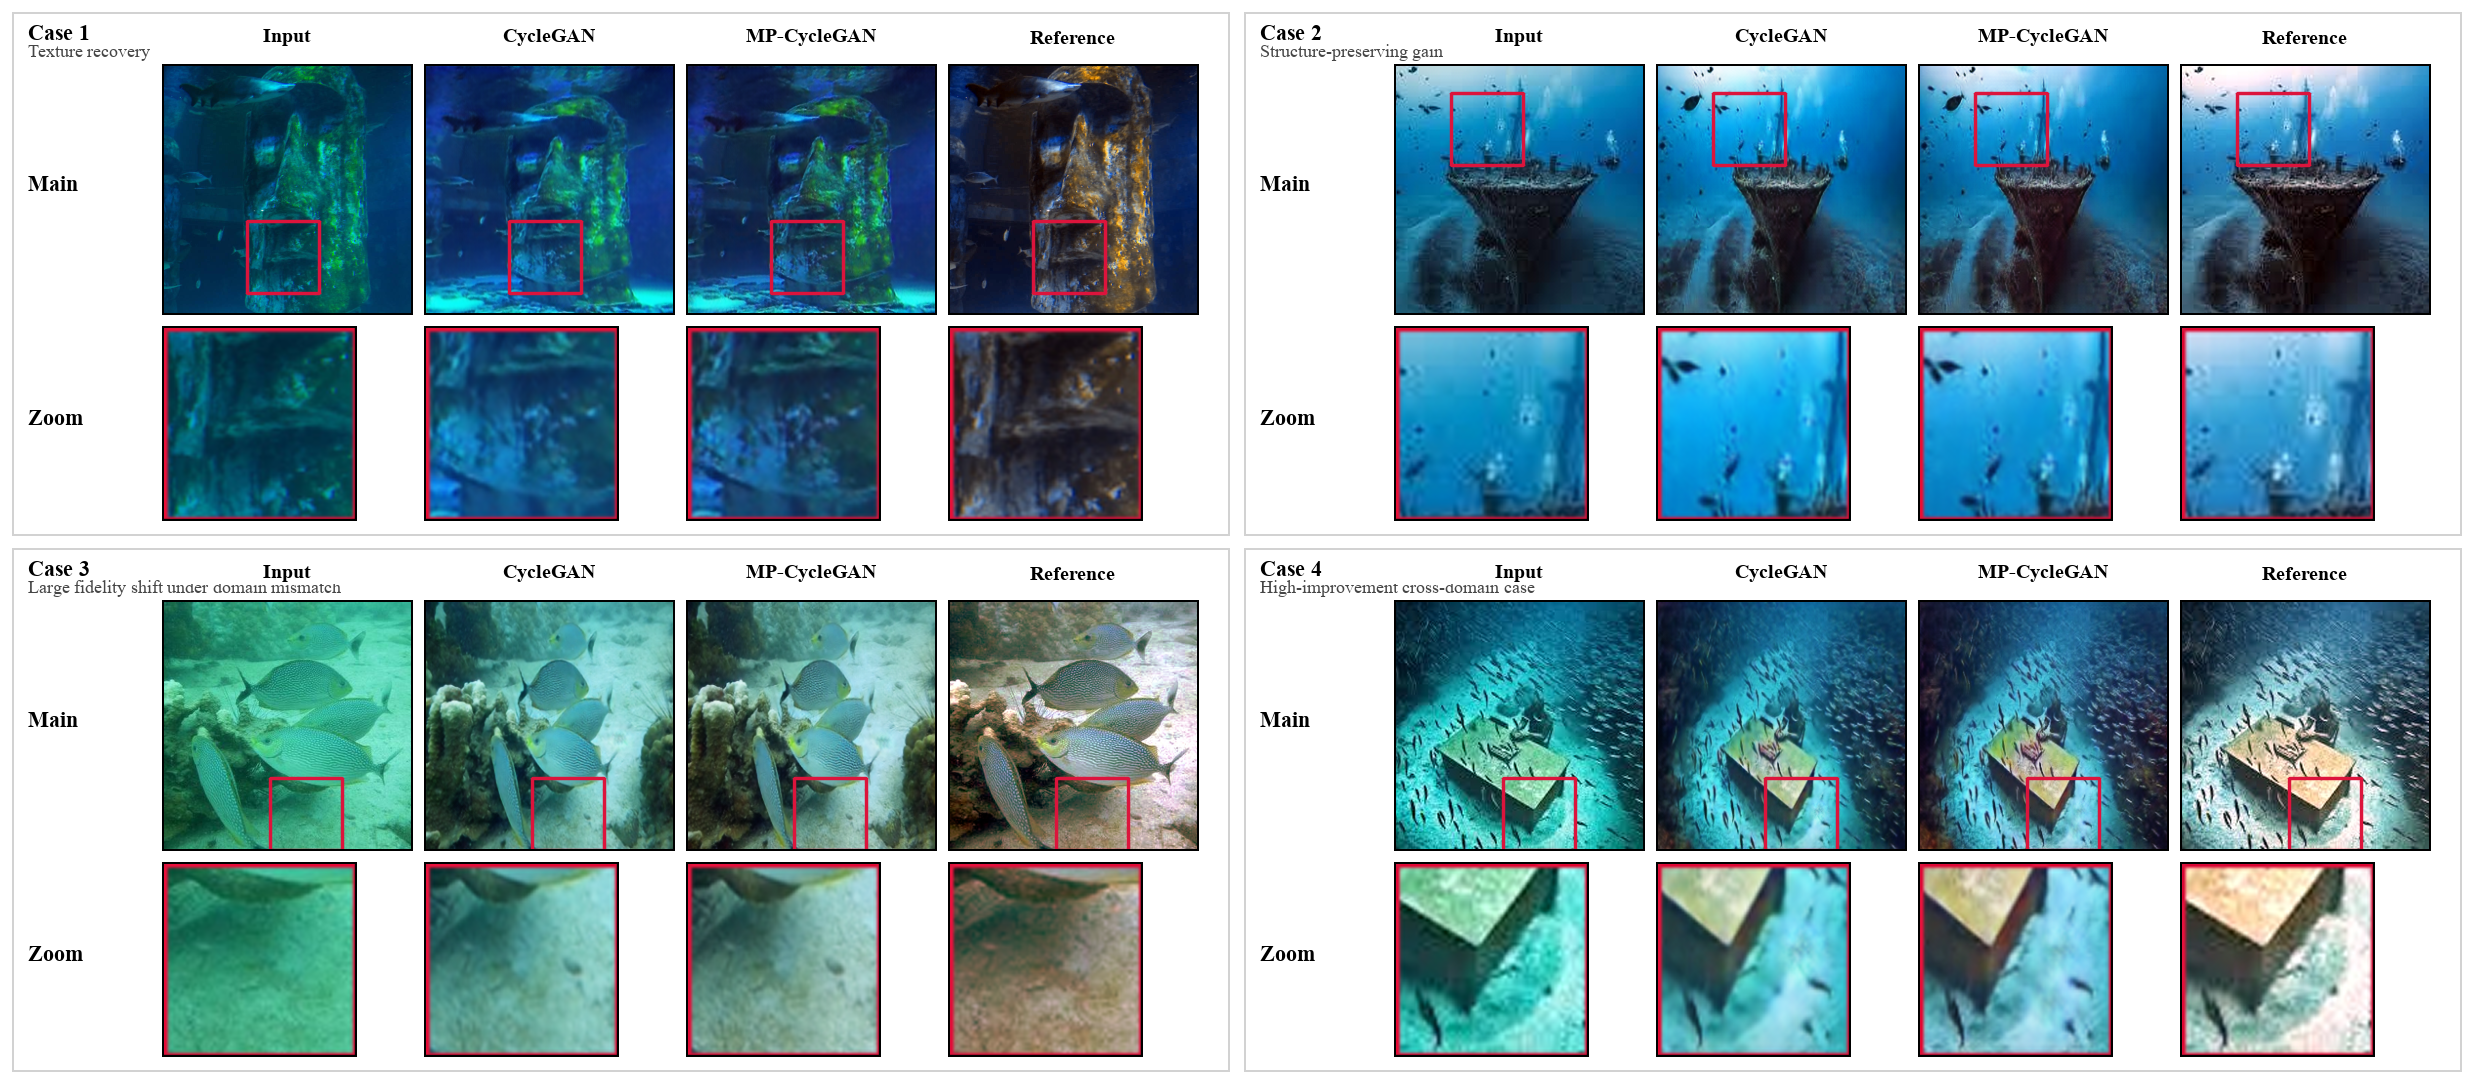
\includegraphics[width=0.95\linewidth]{figures_used/Fig3_uieb_cross_domain_qualitative_spic.png}
\caption{Cross-domain qualitative results on UIEB (EUVP-trained same-budget 250 models tested on UIEB). The figure shows representative UIEB cases identified from paired per-image analysis, together with the matched reference column to make the cross-domain fidelity shift visually identifiable.}
\end{figure}

\subsection{Ablation Study (UIEB Subset)}
To isolate the contribution of each MP component under a controlled small-budget setting, we conduct an ablation on UIEB using 20 training epochs and a capped training set (\texttt{max\_dataset\_size=200}). Evaluation is performed on a matched subset of 50 pairs for efficiency. The purpose of this study is to examine directional trends among the constraints rather than to replace the main EUVP-based training protocol. Configurations are: (A) CycleGAN; (B) +gray-world; (C) +gray-world +structure; (D) +gray-world +structure +perceptual; (E) +gray-world +structure +perceptual +auxiliary color statistics.

\begin{table}[!t]
\centering
\caption{Ablation results on UIEB matched subset (matched=50). PSNR/SSIM are reported as mean $\pm$ half-width of the 95\% bootstrap CI.}
\begin{tabular}{lccccccc}
\toprule
Config & $\mathcal{L}_{gray}$ & $\mathcal{L}_{struct}$ & $\mathcal{L}_{perc}$ & PSNR (dB) & SSIM & UCIQE & UIQM \\
\midrule
A (Base) &  &  &  & 17.41$\pm$0.63 & 0.495$\pm$0.027 & 27.89 & 8.01 \\
B & $\checkmark$ &  &  & 17.63$\pm$0.67 & 0.495$\pm$0.025 & \textbf{28.82} & 8.19 \\
C & $\checkmark$ & $\checkmark$ &  & 16.86$\pm$0.57 & 0.566$\pm$0.026 & 27.21 & 9.01 \\
D (Ours) & $\checkmark$ & $\checkmark$ & $\checkmark$ & \textbf{18.30$\pm$0.65} & \textbf{0.584$\pm$0.022} & 28.44 & 9.34 \\
E$^\dagger$ & $\checkmark$ & $\checkmark$ & $\checkmark$ & 16.95$\pm$0.63 & 0.572$\pm$0.024 & 27.63 & \textbf{9.42} \\
\bottomrule
\end{tabular}
\vspace{2pt}

\footnotesize
$\dagger$ Configuration E includes the auxiliary color-statistics regularizer, which improves no-reference metrics but weakens the full-reference operating point.
\end{table}

The ablation reveals a consistent qualitative pattern. Adding the gray-world term improves color-oriented quality, adding the structure term mainly benefits SSIM, and adding the perceptual term yields the best joint PSNR/SSIM result in this small-budget setting. The auxiliary color-statistics term further increases UIQM but slightly weakens PSNR/SSIM, which supports our decision not to include it in the default MP-CycleGAN definition. Because this ablation is intentionally budget-limited, we treat it as evidence of module tendencies rather than a definitive ranking under the full training schedule.

\begin{figure}[!t]
\centering
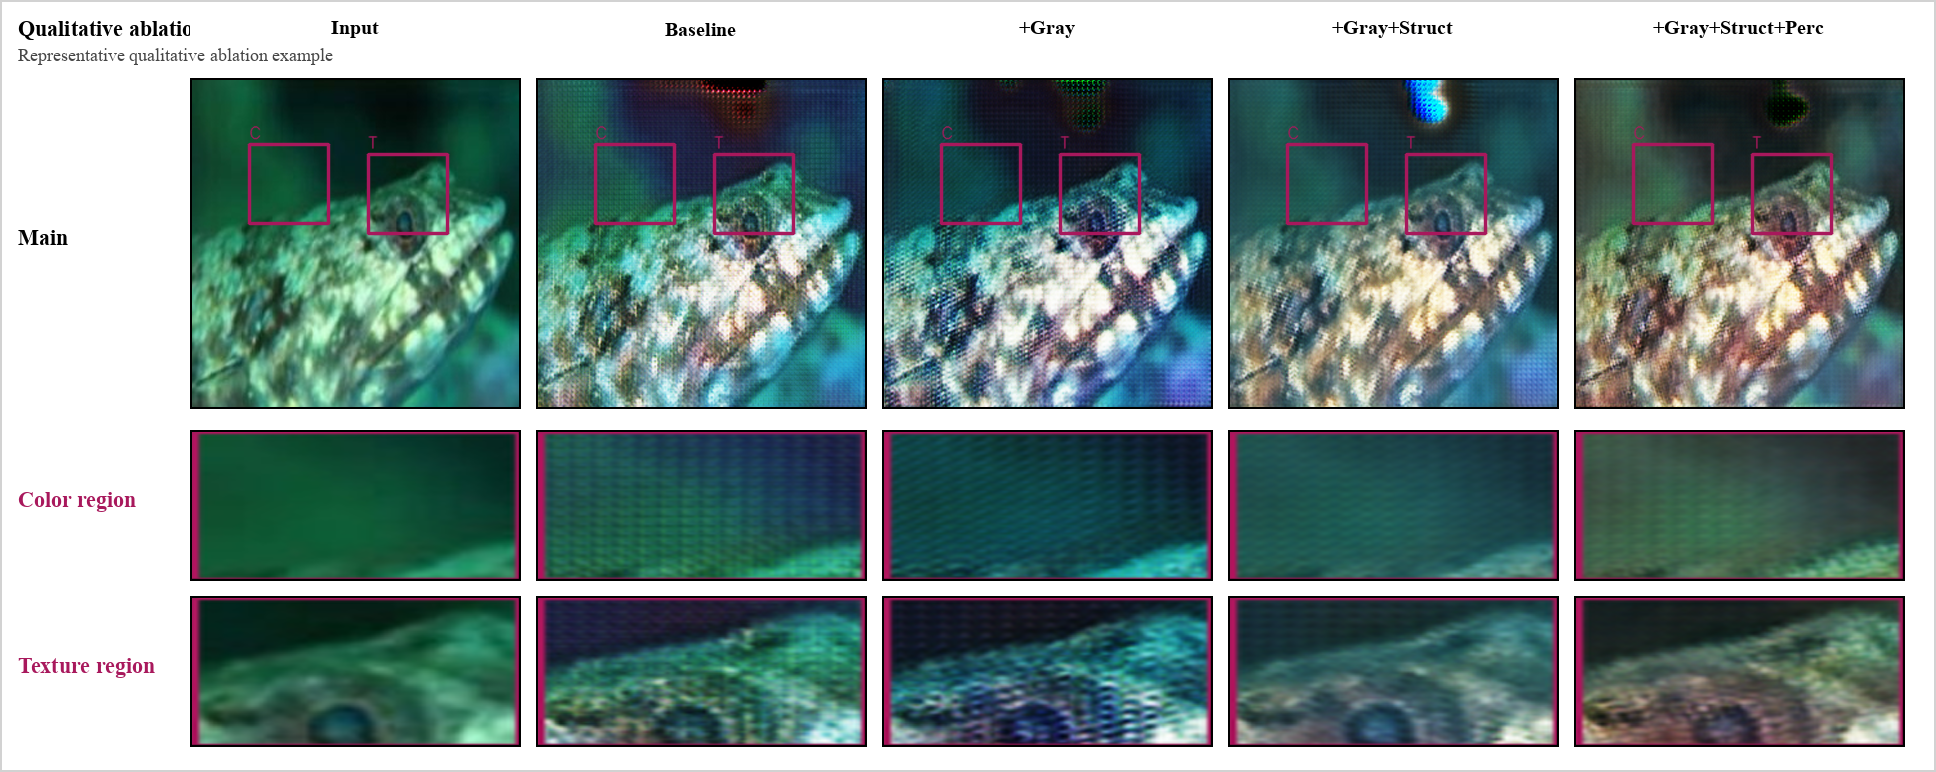
\includegraphics[width=0.95\linewidth]{figures_used/Fig4_ablation_visualization_spic.png}
\caption{Qualitative ablation example under the small-budget UIEB setting. From left to right, the columns show the input, baseline, +gray, +gray+struct, and +gray+struct+perc configurations. The highlighted regions emphasize the trade-off between color stabilization and texture preservation.}
\end{figure}

\subsection{Additional Visual Analysis}
\begin{figure}[!t]
\centering
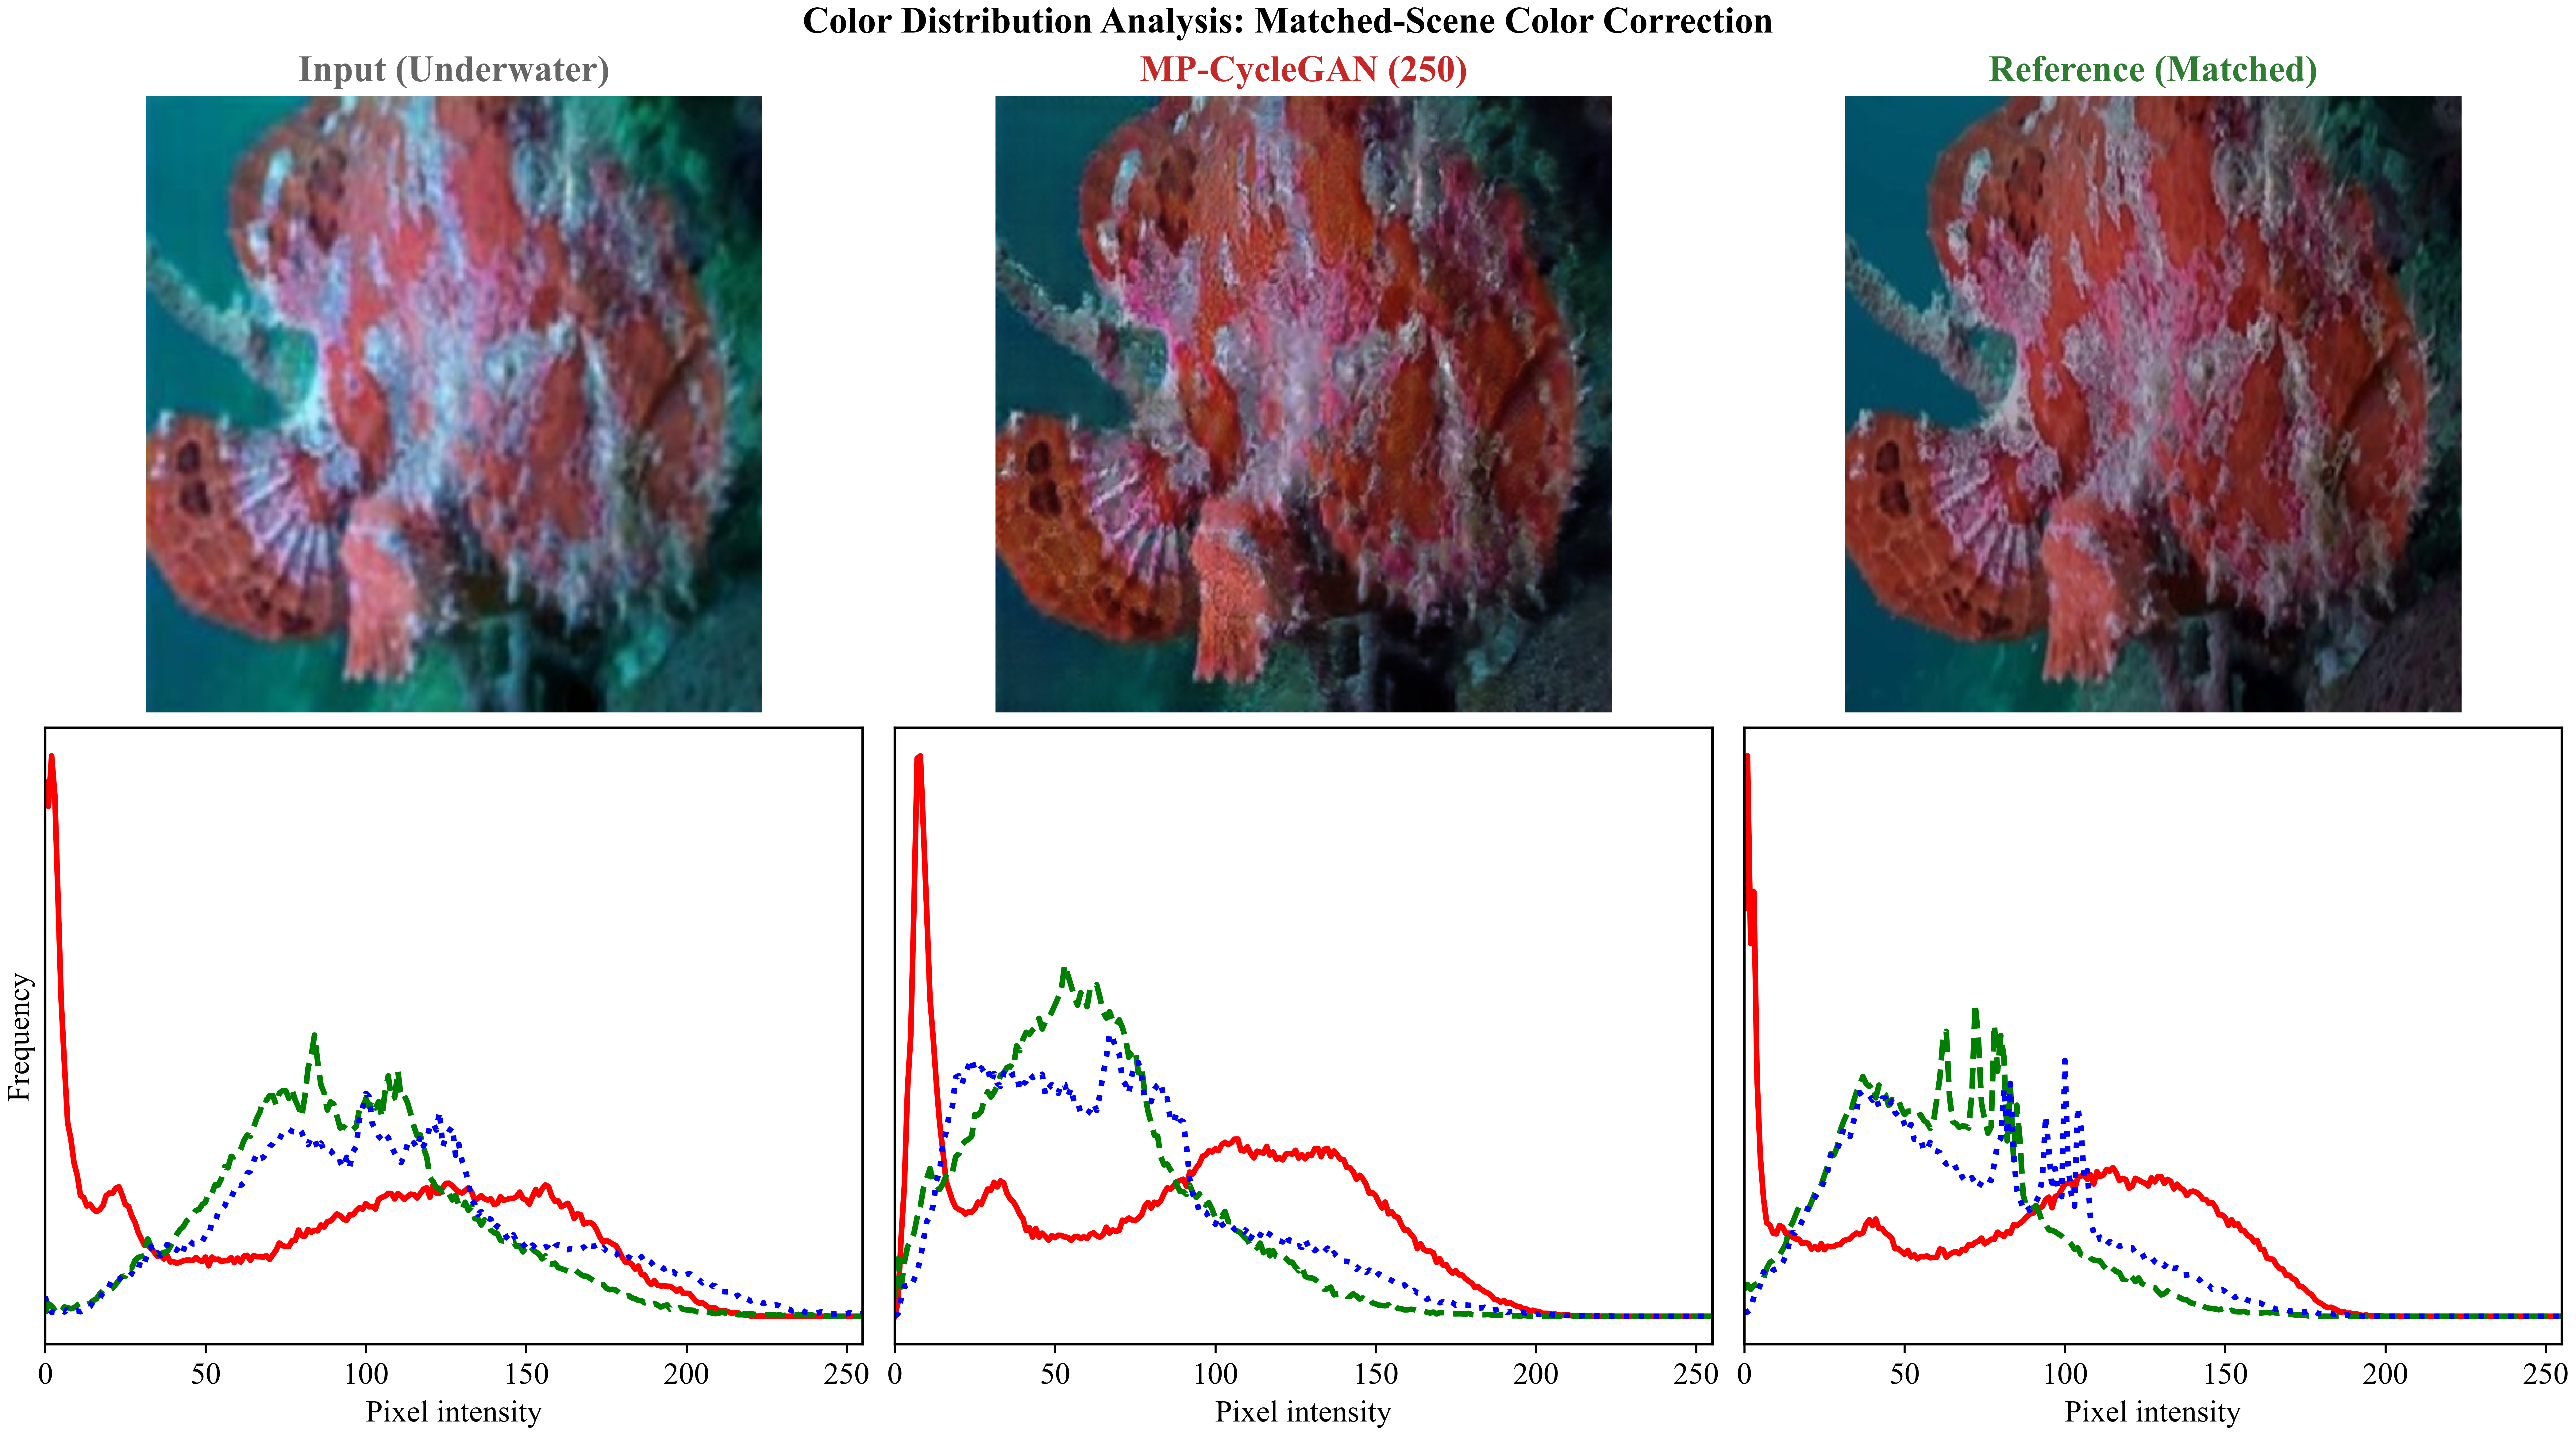
\includegraphics[width=0.92\linewidth]{figures_used/color_distribution_analysis.png}
\caption{Matched-scene color-distribution analysis for a representative EUVP example. The figure compares the input, the final MP-CycleGAN (epoch250) output, and the matched reference, and visualizes the associated RGB histogram shift using color and line-style coding.}
\end{figure}

The color-distribution figure provides an additional view of the visual behavior discussed above. In particular, it shows on a matched-scene EUVP example that MP-CycleGAN reduces blue/green dominance and shifts the red channel toward the reference distribution without forcing all channels toward an identical histogram shape. This observation is consistent with the qualitative examples in the in-domain and cross-domain result sections: the proposed constraints encourage more balanced color correction, but the resulting trade-off still depends on scene content and domain shift.

\subsection{Downstream Detection (Domain-Shift Analysis)}
To assess practical utility beyond image-quality metrics, we additionally evaluate underwater object detection performance on a labeled underwater detection dataset using a YOLO-based detector. We use the URPC optical object detection dataset~\cite{urpc2020} with four common underwater classes (holothurian, echinus, scallop, starfish). We evaluate detection on the original validation images and their MP-CycleGAN enhanced counterparts while keeping labels identical. This experiment is intended to probe domain shift, not to claim that enhancement automatically improves any frozen detector. We therefore report three settings: a detector trained on raw images only, a detector adapted to enhanced images, and a mixed detector trained on both raw and enhanced data.
The detection analysis (Table~\ref{tab:urpc_det} and Fig.~\ref{fig:urpc_det}) confirms that enhancement changes the image distribution seen by the detector. A detector trained only on raw images degrades substantially on enhanced inputs, while mixed or enhancement-aware training partially recovers performance. For the present paper, this result is best interpreted as evidence that UIE quality and downstream model compatibility should be analyzed jointly rather than assumed to be automatically aligned.

\begin{table}[!t]
\centering
\caption{Downstream object detection performance on URPC optical (validation split).}
\label{tab:urpc_det}
\begin{tabular}{lcc}
\toprule
Detector \& Validation Domain & mAP@0.5 & mAP@0.5:0.95 \\
\midrule
\multicolumn{3}{l}{\textbf{Fixed Detector (Trained on raw images)}} \\
Raw Validation & 0.8365 & 0.4908 \\
MP-CycleGAN Enhanced & 0.4614 & 0.2157 \\
\midrule
\multicolumn{3}{l}{\textbf{Enhancement-Aware Detector (Adapted to enhanced domain)}} \\
Raw Validation & 0.5787 & 0.2672 \\
MP-CycleGAN Enhanced & 0.6261 & 0.3181 \\
\midrule
\multicolumn{3}{l}{\textbf{Mixed Detector (Trained on raw + enhanced data)}} \\
Raw Validation & $0.8458\pm0.0005$ & $0.4982\pm0.0011$ \\
MP-CycleGAN Enhanced & $0.6601\pm0.0034$ & $0.3388\pm0.0003$ \\
\bottomrule
\end{tabular}
\end{table}

\begin{figure}[!t]
\centering
\includegraphics[width=\linewidth]{figures_used/downstream_detection_fixed_vs_mixed.png}
\caption{Qualitative downstream detection comparison on URPC (top: fixed detector trained on raw; bottom: mixed detector trained on raw and MP-CycleGAN enhanced images). Green: ground-truth boxes. Red: predicted boxes.}
\label{fig:urpc_det}
\end{figure}

\section{Discussion and Limitations}
MP-CycleGAN improves the stability of unpaired enhancement by combining complementary constraints, but several limitations remain. First, the measured in-domain gains over CycleGAN are limited in magnitude, and the paired analysis shows that the clearest positive signal under the final same-budget control is on PSNR rather than on SSIM; the method should therefore be viewed as a regularized refinement of a strong baseline rather than a replacement of the underlying architecture. Second, although the current UIEB export shows modest positive shifts in PSNR and SSIM, the cross-domain results still highlight a mismatch between full-reference and no-reference criteria; this indicates that current UIE benchmarks do not fully resolve the gap between reference similarity and deployment-oriented perceptual usefulness. Third, the downstream detection experiment shows that enhancement can introduce distribution shift for a detector trained only on raw images. In other words, better-looking images do not automatically translate into better machine-vision performance unless the detector is adapted to the enhanced domain. Finally, the current MP design uses fixed loss weights and a single backbone, and the UIEB paired analysis also required excluding 23 rows with missing full-reference values, so adaptive weighting, stronger same-budget controls, and more robust benchmark tooling remain open directions.

\section{Conclusion}
We presented MP-CycleGAN for unpaired underwater image enhancement. Rather than redesigning the generator, the method regularizes a standard CycleGAN backbone with gray-world, gradient-consistency, and perceptual constraints during training only. Under a unified evaluation protocol with a same-budget continuation control from epoch200 to epoch250, the resulting model shows a modest but statistically supported in-domain PSNR refinement on the full EUVP matched subset, a modest cross-domain PSNR/SSIM improvement on the 841-image UIEB matched subset together with mixed no-reference trends, and the same inference-time complexity as the baseline backbone. The main finding is therefore intentionally narrow: lightweight training-time regularization can improve the fidelity stability of an unpaired UIE pipeline without adding inference-time cost, but the practical value of enhancement must still be judged jointly through matched-set fidelity, cross-domain trade-offs, and downstream compatibility. Future work should emphasize adaptive constraint weighting, broader comparisons with newer UIE paradigms, tighter coupling between enhancement and task-aware evaluation, and more robust benchmark handling for incomplete metric rows.

\section*{Declaration of competing interest}
The authors declare that they have no known competing financial interests or personal relationships that could have appeared to influence the work reported in this paper.

\section*{Funding}
This work was supported by the Yunnan Provincial Basic Research General Program (Grants 202601AT070017 and 202301AT070065).

\section*{Data availability}
EUVP and UIEB datasets are publicly available. The project codebase associated with this study is available at \url{https://github.com/aaziqi/haimou-zhiche}. The training scripts, evaluation scripts, configuration files, figure assets, and benchmark summaries used for this manuscript are organized in the public repository and will be maintained as a reproducibility-focused release for this study.

\section*{CRediT authorship contribution statement}
Aoqi Li: Conceptualization, Methodology, Software, Formal analysis, Data curation, Visualization, Writing -- original draft. 
Rongzhi Yang: Investigation, Resources, Validation, Writing -- review \& editing. 
Zixuan Yang: Data curation, Validation, Formal analysis, Writing -- review \& editing. 
Chenfu Yang: Supervision, Project administration, Funding acquisition, Writing -- review \& editing.

\section*{Declaration of generative AI and AI-assisted technologies in the manuscript preparation process}
During the preparation of this work the authors used Trae (an AI-assisted IDE) to draft parts of the code and to assist literature lookup and method exploration. After using this tool, the authors reviewed and edited the content as needed and take full responsibility for the content of the published article.

\section*{Acknowledgements}
The authors thank the maintainers of the EUVP, UIEB, and URPC datasets for making their benchmarks publicly available.

\begin{thebibliography}{99}
\bibitem{zhu2017cyclegan} J.-Y. Zhu, T. Park, P. Isola, and A. A. Efros, ``Unpaired Image-to-Image Translation Using Cycle-Consistent Adversarial Networks,'' in \emph{Proc. ICCV}, 2017, pp. 2242--2251.
\bibitem{chiang2012wavelength} J. Y. Chiang and Y.-C. Chen, ``Underwater Image Enhancement by Wavelength Compensation and Dehazing,'' \emph{IEEE Transactions on Image Processing}, vol. 21, no. 4, pp. 1756--1769, 2012.
\bibitem{ancuti2012fusion} C. Ancuti, C. O. Ancuti, T. Haber, and P. Bekaert, ``Enhancing Underwater Images and Videos by Fusion,'' in \emph{Proc. IEEE Conf. Comput. Vis. Pattern Recognit.}, 2012, pp. 81--88.
\bibitem{peng2017blurriness} Y.-T. Peng and P. C. Cosman, ``Underwater Image Restoration Based on Image Blurriness and Light Absorption,'' \emph{IEEE Transactions on Image Processing}, vol. 26, no. 4, pp. 1579--1594, 2017.
\bibitem{akkaynak2019seathru} D. Akkaynak and T. Treibitz, ``Sea-Thru: A Method for Removing Water from Underwater Images,'' in \emph{Proc. IEEE/CVF Conf. Comput. Vis. Pattern Recognit.}, 2019, pp. 1682--1691.
\bibitem{li2020uieb} C. Li, C. Guo, W. Ren, R. Cong, J. Hou, S. Kwong, and D. Tao, ``An Underwater Image Enhancement Benchmark Dataset and Beyond,'' \emph{IEEE Transactions on Image Processing}, vol. 29, pp. 4376--4389, 2020.
\bibitem{islam2020funiegan} M. J. Islam, Y. Xia, and J. Sattar, ``Fast Underwater Image Enhancement for Improved Visual Perception,'' \emph{IEEE Robotics and Automation Letters}, vol. 5, no. 2, pp. 3227--3234, 2020.
\bibitem{li2021ucolor} C. Li, S. Anwar, J. Hou, R. Cong, C. Guo, and W. Ren, ``Underwater Image Enhancement via Medium Transmission-Guided Multi-Color Space Embedding,'' \emph{IEEE Transactions on Image Processing}, vol. 30, pp. 4985--5000, 2021.
\bibitem{park2024asnet} C. W. Park and I. K. Eom, ``Underwater image enhancement using adaptive standardization and normalization networks,'' \emph{Engineering Applications of Artificial Intelligence}, vol. 127, Art. no. 107445, 2024.
\bibitem{zhang2024cnms} D. Zhang, C. Wu, J. Zhou, W. Zhang, Z. Lin, K. Polat, and F. Alenezi, ``Robust underwater image enhancement with cascaded multi-level sub-networks and triple attention mechanism,'' \emph{Neural Networks}, vol. 169, pp. 685--697, 2024.
\bibitem{tang2023diffusion} Y. Tang, H. Kawasaki, and T. Iwaguchi, ``Underwater Image Enhancement by Transformer-based Diffusion Model with Non-uniform Sampling for Skip Strategy,'' in \emph{Proc. ACM Multimedia}, 2023, pp. 5419--5427.
\bibitem{ding2025aldiff} X. Ding, X. Chen, Y. Sui, Y. Wang, and J. Zhang, ``Underwater Image Enhancement Using a Diffusion Model with Adversarial Learning,'' \emph{Journal of Imaging}, vol. 11, no. 7, Art. no. 212, 2025.
\bibitem{liu2024zerouae} T. Liu, K. Zhu, X. Wang, W. Song, and H. Wang, ``Lightweight Underwater Image Adaptive Enhancement Based on Zero-reference Parameter Estimation Network,'' \emph{Frontiers in Marine Science}, vol. 11, 2024, Art. no. 1378817.
\bibitem{fabbri2018ugan} C. Fabbri, M. J. Islam, and J. Sattar, ``Enhancing Underwater Imagery Using Generative Adversarial Networks,'' in \emph{Proc. IEEE Int. Conf. Robot. Autom.}, 2018, pp. 7159--7165.
\bibitem{jia2024unsupervised} Y. Jia, Z. Wang, L. Zhao, ``An Unsupervised Underwater Image Enhancement Method Based on Generative Adversarial Networks with Edge Extraction,'' \emph{Frontiers in Marine Science}, vol. 11, 2024, Art. no. 1471014.
\bibitem{wang2024sagan} H. Wang, M. Yang, G. Yin, and J. Dong, ``Self-Adversarial Generative Adversarial Network for Underwater Image Enhancement,'' \emph{IEEE Journal of Oceanic Engineering}, vol. 49, no. 1, pp. 237--248, 2024.
\bibitem{johnson2016perceptual} J. Johnson, A. Alahi, and L. Fei-Fei, ``Perceptual Losses for Real-Time Style Transfer and Super-Resolution,'' in \emph{Proc. ECCV}, 2016.
\bibitem{buchsbaum1980grayworld} G. Buchsbaum, ``A Spatial Processor Model for Object Colour Perception,'' \emph{Journal of the Franklin Institute}, vol. 310, no. 1, pp. 1--26, 1980.
\bibitem{cong2024survey} X. Cong, Y. Zhao, J. Gui, J. Hou, and D. Tao, ``A Comprehensive Survey on Underwater Image Enhancement Based on Deep Learning,'' arXiv:2405.19684, 2024.
\bibitem{lai2025review} Y. L. Lai, T. F. Ang, U. A. Bhatti, C. S. Ku, Q. Han, and L. Y. Por, ``Color Correction Methods for Underwater Image Enhancement: A Systematic Literature Review,'' \emph{PLOS ONE}, vol. 20, no. 3, e0317306, 2025.
\bibitem{shen2025uiqe} M. Shen, M. Yang, J. Zhong, H. Liu, and C. Pan, ``Underwater Image Quality Evaluation: A Comprehensive Review,'' \emph{IET Image Processing}, vol. 19, no. 1, e70068, 2025.
\bibitem{liu2024uiqa} Y. Liu, B. Zhang, R. Hu, K. Gu, G. Zhai, and J. Dong, ``Underwater Image Quality Assessment: Benchmark Database and Objective Method,'' \emph{IEEE Transactions on Multimedia}, vol. 26, pp. 7734--7747, 2024.
\bibitem{urpc2020} URPC, ``Underwater Robot Picking Competition (Optical Image Object Detection) Dataset,'' 2020. [Online]. Available: \url{https://openi.pcl.ac.cn/OpenOrcinus_orca/URPC_opticalimage_dataset/datasets}.
\bibitem{wang2004ssim} Z. Wang, A. C. Bovik, H. R. Sheikh, and E. P. Simoncelli, ``Image Quality Assessment: From Error Visibility to Structural Similarity,'' \emph{IEEE Transactions on Image Processing}, vol. 13, no. 4, pp. 600--612, 2004.
\bibitem{yang2015uciqe} M. Yang and A. Sowmya, ``An Underwater Color Image Quality Evaluation Metric,'' \emph{IEEE Transactions on Image Processing}, vol. 24, no. 12, pp. 6062--6071, 2015.
\bibitem{panetta2016uiqm} K. Panetta, C. Gao, and S. Agaian, ``Human-Visual-System-Inspired Underwater Image Quality Measures,'' \emph{IEEE Journal of Oceanic Engineering}, vol. 41, no. 3, pp. 541--551, 2016.
\bibitem{simonyan2015vgg} K. Simonyan and A. Zisserman, ``Very Deep Convolutional Networks for Large-Scale Image Recognition,'' in \emph{Proc. ICLR}, 2015.
\end{thebibliography}

\end{document}
